% autore: Andrea Ciprietti

\createsection{\MlogM}{{\small{$\blacksquare$}} \normalsize Implementazione in \texttt{C++11}}
    
    Si richiede di determinare il più lungo cammino formato da archi con pesi strettamente crescenti in un grafo diretto (non necessariamente aciclico o connesso), in cui i nodi rappresentano gli $N$ incroci e gli archi le $M$ strade. Nel seguito, descriviamo una soluzione che utilizza un approccio in linea di massima \textit{greedy} -- vale a dire, tale che la soluzione globale ottima si ottiene da un insieme di scelte locali anch'esse ottimali.
    
    Per comprendere meglio l'algoritmo che stiamo per illustrare, si consideri anzitutto una versione semplificata del problema, in cui gli archi (cioè le strade) hanno tutti pesi (lunghezze) diversi. Dopo aver ordinato gli archi in ordine \textit{decrescente} di peso, in un array \texttt{memo} si mantiene la lunghezza massima tra tutti i cammini crescenti che partono da un certo nodo\footnote{Inizialmente, si assume che il massimo cammino che parte da ogni nodo abbia lunghezza nulla, pertanto si avrà che $\texttt{memo[$i$]} = 0 \; \; \forall \; 0 \le i < N$.}. Alla $i$-esima iterazione dell'algoritmo, si estrae dalla lista ordinata l'arco $(u_i, \: v_i)$ e si aggiorna il valore di \texttt{memo[$u_i$]} -- nel caso in cui quello precedente fosse minore di $\texttt{memo[$v_i$]} + 1$ -- sostituendolo con quest'ultimo. Alla fine, sarà sufficiente ritornare il valore massimo memorizzato in \texttt{memo}.
    
    Questa soluzione potrebbe produrre un output errato se alcune strade possiedono la medesima lunghezza. Infatti, è possibile che a un certo cammino venga aggiunto un arco di peso uguale a quello iniziale di tale percorso: ovviamente, in questo modo vengono considerati anche i cammini \textit{debolmente} crescenti, ergo il valore restituito potrebbe essere maggiore di quello atteso.
    
    Per poter risolvere il caso generale, è necessario apportare qualche modifica all'algoritmo iniziale. Come prima, si ordinano gli archi in ordine decrescente di peso. Questa volta, tuttavia, si estraggono ``a gruppi'', aggiornando in una volta tutti gli archi aventi stesso peso. La differenza principale con la soluzione precedente sta nel fatto che l'aggiornamento non avverrà direttamente all'interno di \texttt{memo}, ma sarà preceduto da una fase di transito, durante la quale i nuovi valori verranno memorizzati temporaneamente in un array \texttt{aggiornamento}. Solo dopo aver processato tutti gli archi di uno stesso gruppo, le soluzioni intermedie verranno trasferite in \texttt{memo}. La \figurename~\ref{fig2} (a pagina seguente) servirà a chiarire il concetto.
    
    \begin{figure}[ht]
        \begin{center}
            \begin{minipage}[t]{0.3\textwidth}
                \asyinclude{asy_velox/fig_2a}
                (a)
                
                ~
            \end{minipage}
            \begin{minipage}[t]{0.3\textwidth}
                \asyinclude{asy_velox/fig_2b}
                (b)
                
                ~
            \end{minipage}
            \begin{minipage}[t]{0.3\textwidth}
                \asyinclude{asy_velox/fig_2c}
                (c)
                
                ~
            \end{minipage}
            \begin{minipage}[t]{0.3\textwidth}
                \asyinclude{asy_velox/fig_2d}
                (d)
            \end{minipage}
            \begin{minipage}[t]{0.3\textwidth}
                \asyinclude{asy_velox/fig_2e}
                (e)
            \end{minipage}
            \begin{minipage}[t]{0.3\textwidth}
                \asyinclude{asy_velox/fig_2f}
                (f)
            \end{minipage}
        \end{center}
        \caption{\protect \centering Simulazione dell'esecuzione dell'algoritmo. Nell'immagine 2.f è evidenziato in rosso uno dei due cammini di lunghezza massima.\label{fig2}}
    \end{figure}
    
    È facile convincersi della correttezza di tale algoritmo. È bene, tuttavia, formalizzarne la dimostrazione per induzione.
    \begin{itemize}
        \item Al passo $i = 0$ (ossia prima di aggiungere qualsiasi arco) l'array \texttt{memo} è completamente inizializzato a $0$: possiamo assumere che tale valore sia corretto.
        \item Supponendo che al termine della $i$-esima iterazione tutti i valori memorizzati in \texttt{memo} siano corretti, lo dimostriamo per $i + 1$.
        
        Al grafo viene aggiunto il gruppo di archi aventi la stessa lunghezza $L_{i + 1}$; sia $U_{i + 1}$ l'insieme di tutti i nodi da cui esce almeno uno di questi archi, e -- in modo analogo -- $V_{i + 1}$ l'insieme dei nodi in cui entra almeno uno di essi. Ora, per ogni nodo $u \not \in U_{i + 1}$, il massimo cammino buono che parte da $u$ sicuramente \underline{non} passerà per uno degli archi appena inseriti (dal momento che, se per assurdo vi fosse un percorso crescente che parte da $u$ e attraversa un arco di lunghezza $L_{i + 1}$, allora questo inizierebbe con un arco già presente nel grafo prima della $i + 1$-esima iterazione, e quindi con peso strettamente minore di $L_{i + 1}$), dunque non è necessario aggiornare \texttt{memo[$u$]}.
        
        D'altra parte, se $u$ è un nodo $\in U_{i + 1}$, il nuovo valore di \texttt{memo[$u$]} è pari a \[ \max \{ \texttt{memo[$u$]}, \: \underset{v \in V_{i + 1}}{\max} \{ \texttt{memo[$v$]} + 1 \} \} \] Questo è esattamente ciò che fa l'algoritmo descritto.
    \end{itemize}
    
    Il tempo impiegato per l'ordinamento è $O(M \log M)$, mentre la complessità del corpo centrale dell'algoritmo è $O(M)$: ergo, la complessità è pari a $O(M \log M)$, sufficiente per input dell'ordine di $10^5$.
    
    \newpage
    
    \MlogM
    
    Il codice che proponiamo di seguito fa uso di container del \texttt{C++} e \texttt{C++11} (quali \texttt{map} e \texttt{unordered\_map}) che permettono di eseguire operazioni di inserimento e ricerca in tempo logaritmico (mantenendo quindi la classe di complessità dell'algoritmo a $M \log M$), ma che potrebbero rallentare l'esecuzione del programma. Sebbene, dunque, in gara sia preferibile impiegare strutture dati lineari quali i \textit{vector} o gli array statici, ai fini dell'esemplificazione di cui sotto abbiamo optato per una scelta che predilige la chiarezza e l'eleganza del codice.
    
    \colorbox{white}{\makebox[.99\textwidth][l]{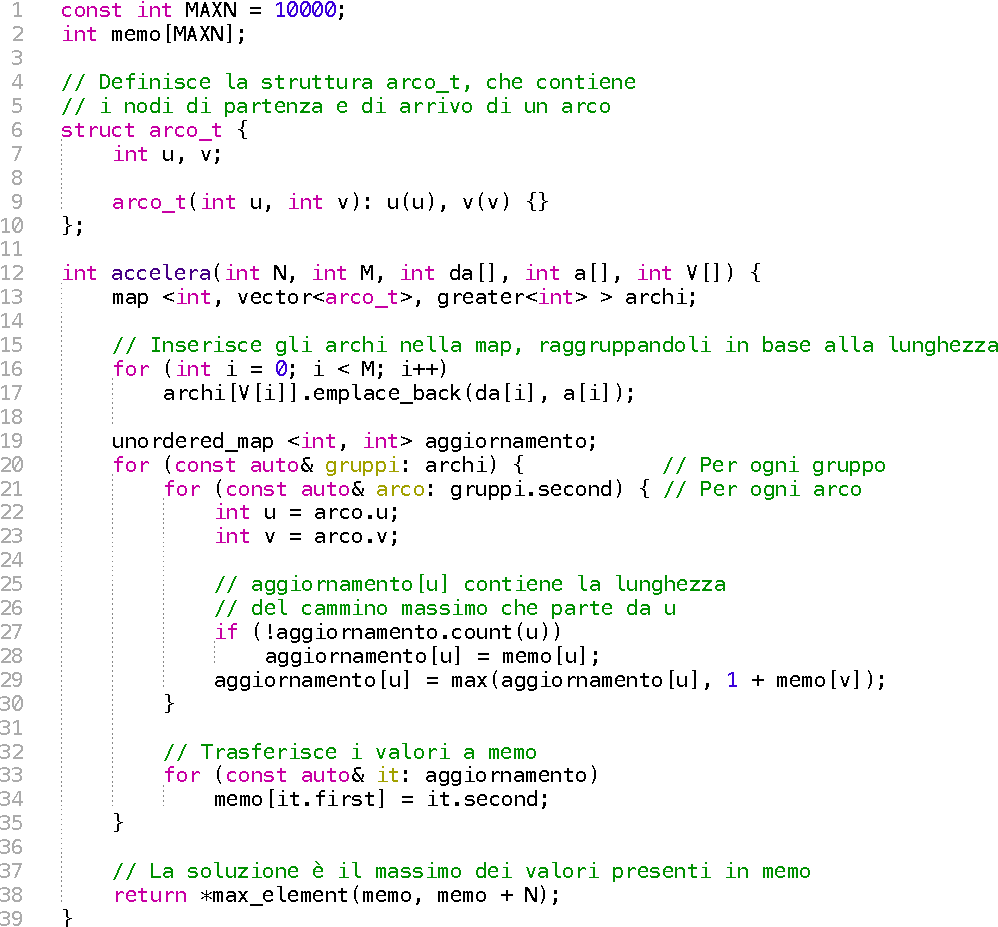
\includegraphics[scale=.8]{velox_mlogm.pdf}}}